\begin{figure}[h]
	\vspace*{-3ex}
	\centering
	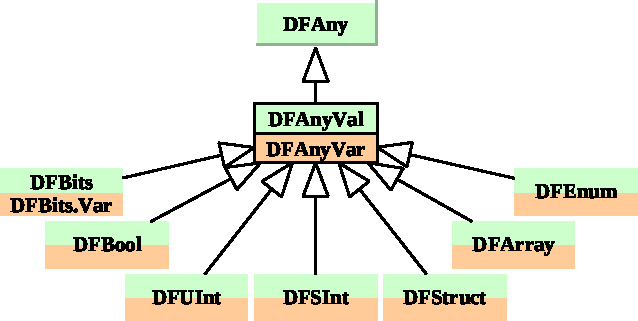
\includegraphics[scale=0.7]{graphics/Inherit.pdf} 
	\captionof{figure}{DFiant dataflow types: simplified inheritance diagram}
	\label{fig:Inherit}
\end{figure}

%\setalgorithmicfont{\small}
\begin{figure*}[h]
  \centering
  \begin{subfigure}[b]{0.5\textwidth}
    \begin{minted}[tabsize=2,gobble=3,frame=single,framesep=2pt, fontsize=\fontsize{7}{8}\selectfont]{Scala}
    class AES_DFKeySchedule(Nk: Int, Nb: Int, Nr : Int) 
      extends AES_DFWords(Nb*(Nr+1)){
      val Rcon = Array[Int](0x00000000, ...)
      def KeyExpansion(key : AES_DFKey): Unit = {
        val temp = AES_DFWord()
      
        for (i <- 0 until Nk)
          this(i) := key(i)
      
      
      
        for (i <- Nk until Nb*(Nr+1)) {
          temp := this(i-1)
          if (i % Nk == 0)
            temp := temp.RotWord().SubWord() ^ Rcon(i / Nk)
          else if ((Nk > 6) && (i % Nk == 4))
            temp := temp.SubWord()
          
          this(i) := this(i-Nk) ^ temp
        
        }
    } }
    \end{minted}
    \caption{DFiant code}
  \end{subfigure}%
%  \hfill
  \begin{subfigure}[b]{0.5\textwidth}
    \begin{minted}[tabsize=2,gobble=3,frame=single,framesep=2pt, fontsize=\fontsize{7}{8}\selectfont]{text}
    //comment line for alignment
    //comment line for alignment
    Rcon = [00000000, ...] 
    KeyExpansion(byte key[4*Nk], word w[Nb*(Nr+1)], Nk) begin
      word temp
      i = 0
      while (i < Nk)
        w[i] = word(key[4*i],key[4*i+1],key[4*i+2],key[4*i+3])
        i = i+1
      end while
      i = Nk
      while (i < Nb * (Nr+1)]
        temp = w[i-1]
        if (i mod Nk = 0)
          temp = SubWord(RotWord(temp)) xor Rcon[i/Nk]
        else if (Nk > 6 and i mod Nk = 4)
          temp = SubWord(temp)
        end if
        w[i] = w[i-Nk] xor temp
        i = i + 1
      end while
    end
    \end{minted}
    \caption{AES spec. pseudo code reference}
  \end{subfigure}
	\vspace*{-4ex}
  \caption{AES KeyExpansion code example}\label{fig:AES}
\end{figure*}

\section{The DFiant Type System}
\label{sec:type_system}
DFiant is a Scala library, hence it inherently supports type safe and rich language constructs. DFiant brings type driven development concepts to hardware design, by creating an extensible dataflow class hierarchy, with the trait \code{DFAny} at its head. 
%(similar concept to Scala's Unified Types hierarchy)
\code{DFAny} contains all properties that are common to every dataflow variable. 
%(e.g., \code{.width} represents the number of bits contained by the variable)
Fig.~\ref{fig:Inherit} illustrates a simplified inheritance diagram of DFiant's dataflow types. 

Fig.~\ref{fig:AES} depicts part of our DFiant Advanced Encryption Standard~\cite{pub2001197} (AES) cipher implementation alongside its specification pseudo code reference. The DFiant code is similar or even simpler in comparison and does not employ global functions. We compared the complete DFiant AES code to three RTL designs~\cite{das2010fully}\cite{hsing2013aes}\cite{salah2013aespipe}. DFiant provides the same functionality with 33-50\% lines of code.
Furthermore, the DFiant code is timing-agnostic and device-agnostic, thus tasking the compiler to construct the hardware fitting the target device and non-functional requirements (e.g., throughput, latency). When constrained by the appropriate target throughput, the DFiant compiler generated an RTL design that acheived better performance than the cited RTL designs.

%Since DFiant is Scala-based, the Scala IDE was utlized for debugging. It was also extremely easy to debug the code step-by-step using
%watches and console printouts. This would have been impossible to do in native HDL
%languages like VHDL and Verilog. After we fixed everything to work in software debugging backend, we have compiled the design to verilog using the hardware construction
%backend, and everything worked in RTL simulation as well.


%The DFiant type system provides the following features:
%\paragraph*{\bf \em Bit-Accurate Operations and Data Structures} 
%All DFiant's dataflow types are bit-accurate and structurally static, with their bit-width set upon construction (e.g., \code{DFBits[5]} is a 5-bit vector). Operations between dataflow variables produce a bit-accurate result with the proper type inference. For example, an addition between an unsigned 5-bit variable (\code{DFUInt[5]}) and a signed 10-bit variable (\code{DFSInt[10]}) produces an adder that can be implicitly converted to a 10-bit signed variable, if carry is not required, or an 11-bit signed variable by explicitly invoking \code{.wc} from the addition.
%
%DFiant also allows operations between dataflow types and their corresponding Scala numeric types, by treating the Scala numeric types as constants (e.g., addition between \code{DFSInt} and \code{Integer} variables). A constant in the dataflow graph is a node that can produce infinite tokens of the same value.   
%
%\paragraph*{\bf \em Mutability} 
%\label{sec:mutability}
%DFiant supports dataflow variables mutability via the \code{:=} operator. Do not confuse with Scala-level mutability which is enabled by using \code{var} instead of \code{val}. Each dataflow class has two variations: an immutable class, which inherits from \code{DFAny\textbf{Val}} and a mutable class, which inherits from \code{DFAny\textbf{Var}} and accepts \code{:=}. The difference between the types enforces an immutable right-hand-side (RHS), where required, and a mutable variable creation. Consider, for instance, the DFiant implementation of \code{g} in Table \ref{tbl:StateExDefImpl}: \code{a} is immutable because it is a RHS addition between the dataflow variable \code{i} and a literal value \code{5}. Contrarily, \code{c} is mutable, since it is a dataflow variable constructor (\code{.init} constructs a new initialized variable, while preserving the mutability trait). 
%
%Fig.~\ref{fig:Inherit} demonstrates a dual class definition for every type  (immutable and mutable). The naming convention helps to reason about the mutability. For example, \code{DFBits} and \code{DFBits.Var} are immutable and mutable classes, respectively. Constructing a new variable via \code{DFBits} (e.g, \code{val a = DFBits[5]}) returns the mutable \code{DFBits.Var[5]}. Usually, we either receive or return an immutable type, hence we do not require annotating a type with its mutable variation. In cases where we want to return a mutable type, we annotate it as an output port (see Section~\ref{sec:io_ports}).
%
%\paragraph*{\bf \em Bit Aliasing and Casting} 
%Aliasing in DFiant enables referencing a part of a dataflow variable, by invoking \code{.bits(hiIdx, loIdx)}, which creates a bits vector alias that references the original variable at the given index parameters. Every change of a dataflow variable affects its alias and vice versa (similar to VHDL's signal aliasing). Since this function also casts the variable as \code{DFBits}, this feature is used as a raw-data cast between different dataflow types. Aliasing of an alias is also possible, while maintaining relative bits indexing. Aliasing preserves the mutability trait: an alias of an immutable variable is immutable, while an alias of a mutable variable is mutable. 
%
%\paragraph*{\bf \em Structural Composition and Generation} 
%
%\begin{figure}[h]
%  \centering
%  \begin{minipage}[b][3cm][b]{0.57\linewidth}
%    \vfill
%    \begin{minted}[xleftmargin=1.5em,linenos,autogobble,tabsize=2,framesep=1pt, frame=single,fontsize=\fontsize{7}{8}\selectfont]{scala}
%      val bits128 = DFBits[128] := 0
%      val alias64 = bits128(127, 64)
%      val alias32 = alias64(31, 0)
%      val dbl = DFDouble := 1.0
%      dbl.bits(7,0) := 0x28
%      bits128(127) := 1
%      bits128(63, 0) := dbl.bits()
%      alias32(16, 8) := 0x57		    
%    \end{minted}
%    \vfill
%    \subcaption{DFiant code}
%  \end{minipage}%
%  \hfill
%  \begin{minipage}[b][3cm][b]{0.40\linewidth}
%    \centering
%    \vfill
%		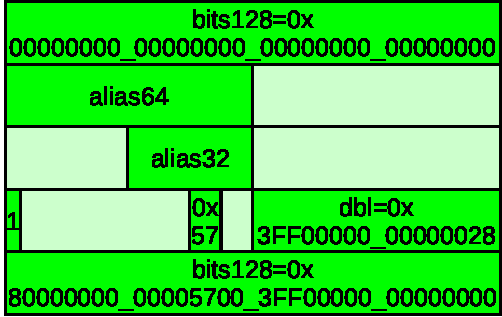
\includegraphics[width=\linewidth]{graphics/Aliasing.pdf} 
%    \vfill
%    \subcaption{Contents of \code{bits128}}
%  \end{minipage}
%  \captionof{figure}{Bit aliasing and casting example}
%  \label{fig:Aliasing}
%\end{figure}
%
%Fig.~\ref{fig:Aliasing} demonstrates aliasing code and its effect on the contents of a dataflow variable (\code{bits128}). Each line code does as follows:
%\begin{enumerate}
%  \item Constructs a new 128-bit vector, \code{bits128}, and clears all its bits.
%  \item Creates a new alias, \code{alias64}, which references the most significant 64 bits of \code{bits128}. Since \code{bits128} is a \code{DFBits} variable, there is no need to invoke \code{.bits()}, and we can apply the required indexes directly.
%  \item Creates a new alias, \code{alias32}, which references the least significant 32 bits of \code{alias64}, which reference bits 64 to 95 of \code{bits128}.
%  \item Constructs a new double precision floating point dataflow variable, \code{dbl}, and initialize its value as \code{1.0} (hexadecimal value of \code{0x3FF00...0}).
%  \item Modifies the least significant byte of \code{dbl}.
%  \item Sets the most significant bit of \code{bits128}.
%  \item Assigns \code{dbl} to the least significant 64 bits of \code{bits128} through casting. All the bits of \code{dbl} are selected because \code{.bits()} is invoked without index parameters.
%  \item Modifies a byte of \code{bits128}.
%  
%\end{enumerate}
%
%
%DFiant expands traditional structural composition capabilities by utilizing Scala's object oriented features such as inheritance and polymorphism, as well as finite loops and recursive composition. The hierarchical compositions provide the scope and dependencies for the dataflow variables. The hierarchy itself is transparent to the dataflow graph, as if the entire design is flattened, inlined, and unrolled. Therefore, hierarchies in DFiant are synthesizable, highly reusable, and do not affect the design performance (may affect compilation time). Different composition examples are available in Table~\ref{tbl:Box}.
%
%\paragraph*{\bf \em IO Ports} 
%\label{sec:io_ports}
%The class \textit{Box} from Table~\ref{tbl:Box} can also be coded as demonstrated in Fig.~\ref{fig:IOBox}. The annotation \code{DFVar $<>$ Dir} controls \textit{DFVar}'s access by encapsulating the variable with the dataflow port class, \code{DFPort}: an \code{IN} port can only be read (immutable), while an \code{OUT} port can only be modified (unreadable). DFiant has implicit conversions in place that selectively converts between \code{DFPort} and \code{DFAny} instances, without breaking mutability rules and type safety. The port annotations match the capabilities of traditional HDLs, and are noticeably absent from HLS languages such as C++. 


